\rhead{\textit{Analysis of the contextual investigation}}
\lhead{}
In this section we will show the results we have obtained from our field surveys and how these results have shaped the requirements of our application.

\subsection{Interviews Answers}
\subsubsection{Interviews with deaf peolple}
We interviewed 5 deaf people who preferred anonymity but gave us permission to use their answers.
 \\ \\
\textbf{First part of the interview (first 5 questions)}: 
3/5 of the interviewed are deaf from birth. The other 2 are becamed deaf as a result of health or congenital problems. \\
In general all of them haven't problems in communication at home, because all their relatives are now able to understand them and make themselves understood and, even without the use of LIS or ASL, the interviewees have become accustomed to reading the labial. \\
Sometimes, with friends and other person, the interviewed had some problems in communication, expecially in being understood. This problem is most visible when they talk with more people at the same time.\\
It rarely happens to fail to understand people, especially when dealing with technical or specialist fields. In those cases it becomes problematic to resume the thread of the speech and this causes them embarrassment.
\\ \\
\textbf{Second Part of the interview (questions 6 - 9)}:
In general they use integrated functionality of their devices, such as signal light to see the notifications and alert systems that take advantage of the vibration, or app like whatsapp, facebook or telegram for doing videocall or texting in place of calls.\\
Some of them have used interpreter, especially when there was a need to speak to many people (for graduation or conference discussions). This gave them more security and allowed them to stay focused. \\
They have not expressed preferences on how the interpreter should speak and in everyday life, and in general, they prefer to speak for themselves.
\\ \\
\textbf{Last part of the interview (last two questions)}:
Some of them rarely used this type of services but they think that this would be a valid help for them, expecially when they attend conferences or frontal lessons where it becomes difficult to follow the interlocutor, who often is at a distance that does not allow lips to be read. But they would not want to use laptops or computers, but would prefer devices for the convenience and size of the device. 
\clearpage
\subsubsection{Interviews with friends and family}
\textbf{First part of the online survey (Questions 1 - 2)}:

\begin{figure}[h]
	\centering
	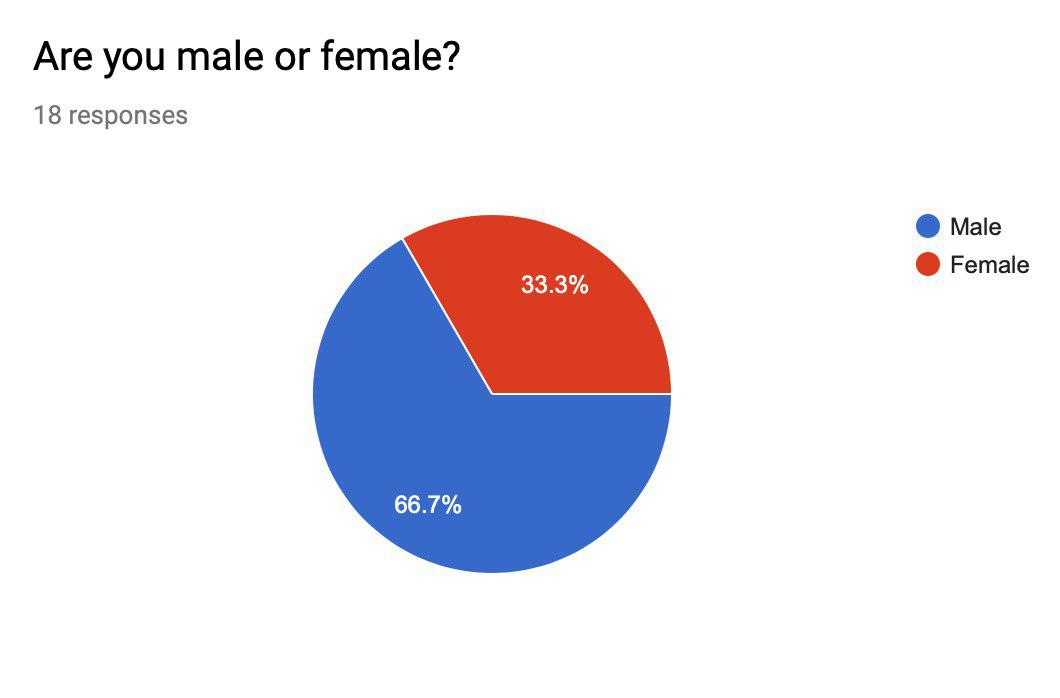
\includegraphics[width=0.7\linewidth]{Figure/photo_2019-02-06_15-58-48}
	\label{fig:photo2019-02-0615-58-48}
\end{figure}
\begin{figure}[h]
	\centering
	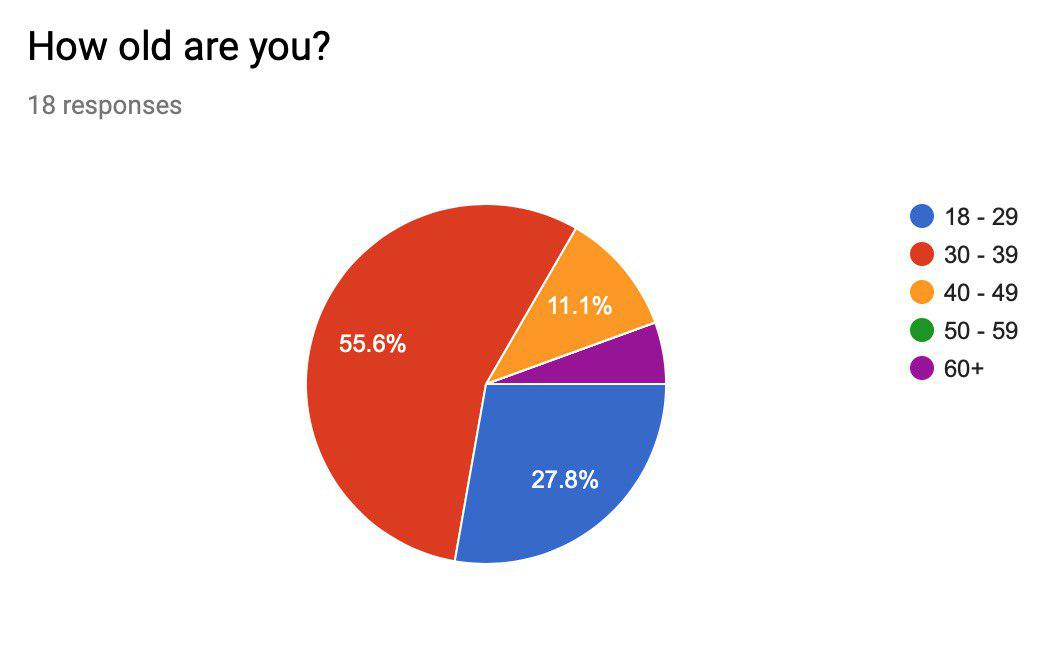
\includegraphics[width=0.7\linewidth]{Figure/photo_2019-02-06_15-58-49}
	\label{fig:photo2019-02-0615-58-49}
\end{figure}
\clearpage
\textbf{Second part of the online survey (Questions 3 - 6)}:
\begin{figure}[h]
	\centering
	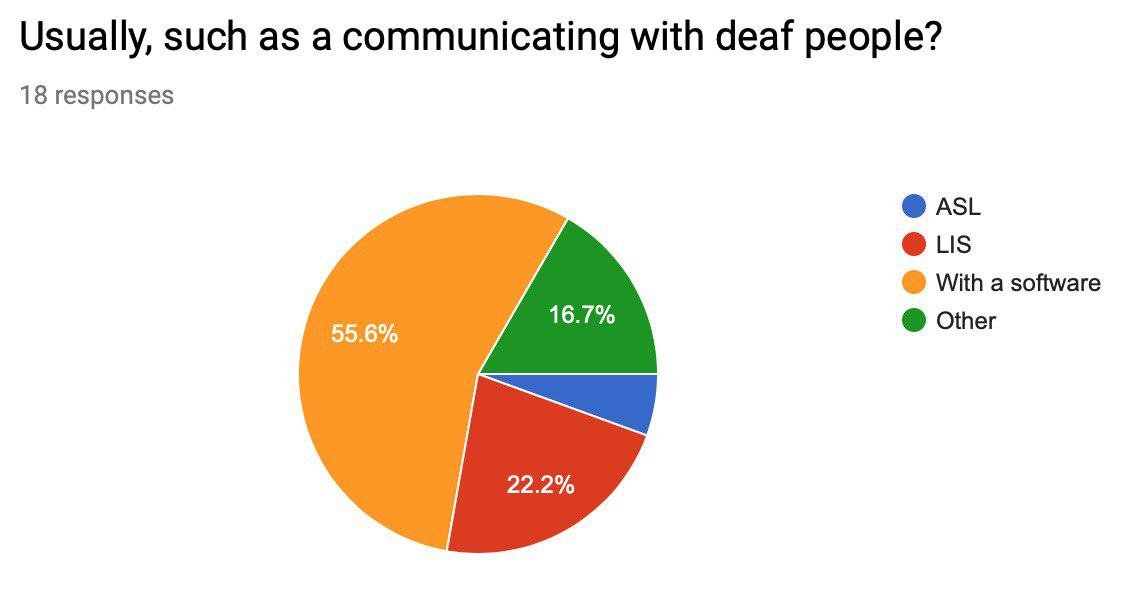
\includegraphics[width=0.7\linewidth]{Figure/photo_2019-02-06_15-58-50}
	\label{fig:photo2019-02-0615-58-50}
\end{figure}
\begin{figure}[h]
	\centering
	\includegraphics[width=0.7\linewidth]{"Figure/photo_2019-02-06_15-58-49 (2)"}
	\label{fig:photo2019-02-0615-58-49-2}
\end{figure}
\begin{figure}[h]
	\centering
	\includegraphics[width=0.7\linewidth]{"Figure/photo_2019-02-06_15-58-50 (2)"}
	\label{fig:photo2019-02-0615-58-50-2}
\end{figure}
\begin{figure}[h]
	\centering
	\includegraphics[width=0.7\linewidth]{"Figure/photo_2019-02-06_15-58-50 (3)"}
	\label{fig:photo2019-02-0615-58-50-3}
\end{figure}
\clearpage
\textbf{Last part of the online survey (Questions 7 - 8)}:

\begin{figure}[h]
	\centering
	\includegraphics[width=0.7\linewidth]{"Figure/photo_2019-02-06_15-58-51 (2)"}
	\label{fig:photo2019-02-0615-58-51-2}
\end{figure}
\begin{figure}[h]
	\centering
	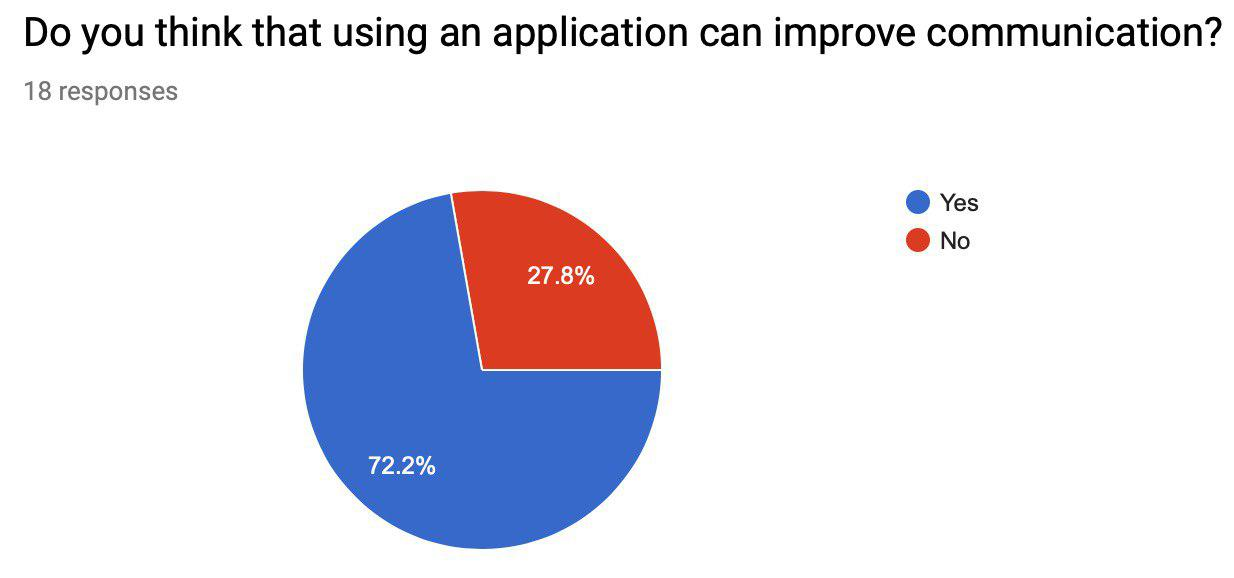
\includegraphics[width=0.7\linewidth]{Figure/photo_2019-02-06_15-58-51}
	\label{fig:photo2019-02-0615-58-51}
\end{figure}

\subsection{Result of the contextual survey}
\subsubsection{Question 1: What activities do users currently perform?}
Some users communicate with a software, others with LIS language and finally others with different systems. Sometimes they have problems in communication and for this reason, whom that don't have applications use different ways for facilitate the communication itself. A lot of people would like to learn LIS or ASL language and use online sites or youtube videos. 

\subsubsection{Question 2: Which tasks would you like to do?}
Users want support for the learning of ASL language and for facilitate the communication.

\subsubsection{Question 3: How are the activities to be learned?}
The main activities to be performed can be learned with a software.

\subsubsection{Question 4: Where are the activities carried out?}
Everywhere, because the only tools neded are internet connection.

\subsubsection{Question 5: What is the relationship between the user and the data (personal data, private data, public data, their meaning for the user, etc.)?}
The user must enter their personal data, they are sensitive data that will be displayed within the application and used to perform certain tasks, such as video calling. However, the user must be aware that his data, even if encrypted, will be subject to the normal security risks of any data that must travel on the network.

\subsubsection{Question 6: What other tools does the user have to complete the task?}
Tools needed are internet connection and online websites to learn ASL and, in some cases, the support of a persone to facilitate the communication.

\subsubsection{Question 7: How often are tasks executed?}
User tasks will be executed whenever there is a communication difficulty. To learn the ASL/LIS, tasks are executed everyday.

\subsubsection{Question 8: What are the time constraints on tasks, if any?}
There are no time constraints on tasks, tasks are constrained solely by the needs of users.

\subsubsection{Question 9: What happens when things go wrong during task execution?}
The communication became complex or in some cases impossible

\subsubsection{Question 10: How do users communicate with each other about tasks?}
Users of tasks communicate in direct way (with ASL/LIS language) or via notifications. For example, if a video call comes in, the device starts to vibrate.